\documentclass[11pt,a4paper]{article}
% rozmery stranky
\usepackage[left=1.5cm,text={18cm, 25cm},top=2.5cm]{geometry}
% cestina a fonty
\usepackage[czech]{babel}
\usepackage[utf8]{inputenc}
\usepackage[T1]{fontenc}
% dalsi balicky
\usepackage{graphicx}
\usepackage{enumitem}
\usepackage{url}
\usepackage[bookmarksopen,colorlinks,plainpages=false,urlcolor=blue,
unicode,linkcolor=black]{hyperref}


\begin{document}

  \begin{titlepage}
    \begin{center}
      \Huge
      \textsc{Fakulta informačních technologií \\ Vysoké učení technické v~Brně}
      \vspace{100px}
      \begin{figure}[!h]
        \centering
        
\includegraphics[height=5cm]{logo}
      \end{figure}
      \\[50mm]
      \LARGE{Tvorba uživatelských rozhraní \,--\, projekt č. 93 \\
             Správa hostingu}
      \vfill
    \end{center}
    \Large{Roman Blanco (xblanc01) - kapitán týmu \hfill 24.10.2014 \\
           Adam Jež (xjezad00)}

  \end{titlepage}

  \section{Abstrakt}

    Cílem zadaného projektu je navrhnout a vytvořit uživatelské rozhraní,
    umožňující uživateli konfigurovat a spravovat své hostingové služby.
    Námi navržené rozhraní by mělo umožňovat správu FTP účtů, DNS
    záznamů, e-mailů a MySQL databází. Ovládání rozhraní navrhujeme tak, aby
    bylo přizpůsobeno jak uživatelům stolních počítačů, tak i uživatelům
    mobilních zařízení, které dokáží zobrazit internetový obsah. Protože naší
    snahou je maximální komfort zákazníků, nejčastěji užívané úkony by měly
    být lehce a rychle proveditelné.

  \section{Úvod}

    V~současnosti již existuje mnoho řešení uživatelských rozhraní pro správu
    hostingu.

    Při vyhledávání inspiračního materiálu jsme se zaměřili na vlastní práci s
    rozhraním - přehledost obsahu, způsob práce s daty a jejich řazení.
    Při návrhu vlastního rozhraní jsme se snažili vyvarovat případných chyb,
    které jsme nalézali v existujících řešeních. Z tohoto hlediska nám
    materiál poskytl jak pozitivní, tak i negativní inspiraci.  Jako studijní
    materiál nám sloužilo především rozhraní webhostingů roští.cz a wedos.cz \\
    \begin{figure}[ht]
      \begin{center}
        \includegraphics[width=12cm]{rosti}
        \caption{Uživatelské rozhraní webhostingu roští.cz}
      \end{center}
    \end{figure}
    \begin{figure}[ht]
      \begin{center}
        \includegraphics[width=12cm]{wedos}
        \caption{Uživatelské rozhraní webhostingu wedos.cz}
      \end{center}
    \end{figure}

  \section{Studium}

    Pro projekt plánujeme použít tyto technologie:
    \begin{description}
      \item[bower] technologie umožňující správu javascriptových knihoven
      \item[less] preprocesor pro CSS
      \item[charts.js] knihovna umožňující jednoduché vytváření grafů
      \item[MySQL] dotazovací jazyk pro získání informací spojené s~uživatelem
      \item[PHP] skriptovací jazyk běžně používaný pro programování
                   dynamických webových stránek
      \item[XML] značkovací jazyk pro popis dokumentu
      \item[XSL] jazyk pro vyjádření stylu
    \end{description}

  %\section{Návrh aplikace}

  \section{Návrh uživatelského rozhraní}

    Našim uživatelským rozhraním bychom chtěli zaujmout také amatérské
    klienty či zákazníky z~menších firem. Oslovit se je budeme snažit
    hlavně jednoduchým a uživatelsky příjemným prostředím se základními funkcemi.
    Naše uživatelské rozhraní by mělo být natolik přívětivé, aby
    jej dokázali ovládat a spravovat i méně zkušení klienti či přímo laici.
    Předpokládáme, že naše cílová skupina nebude zkušena natolik, aby si
    vytvořila vlastní analyzační nástroje, a proto chceme dát možnost použít, mimo jiné,
    užitečné statistiky související s~navštěvováním a používáním hostovaných
    webových stránek.

  \section{Realizace}

    Dosavadní práci na projektu jsme si rozdělili následujícím způsobem:
    \begin{description}
      \item[Roman Blanco] \hfill
        \begin{itemize}
          \item návrh vzhledu rozhraní
          \item zvážení technologií pro použití
          \item vyhledání a nastudování inspiračního materiálu
        \end{itemize}
      \item[Adam Jež:] \hfill
        \begin{itemize}
          \item návrh jednotlivých částí rozhraní
          \item návrh a vytvoření ERD podle návrhu rozhraní
          \item implementace logiky aplikace
        \end{itemize}
    \end{description}


  %\section{Testování}

  %\section{Závěr}

  \section{Reference}

    \begin{enumerate}[label={[\arabic*]}]
      \item repoziář administrace serveru \href{https://github.com/creckx/pcp}{roští.cz}
      \item administrace serveru \href{https://wedos.cz}{wedos.cz}
    \end{enumerate}

  \appendix
  \newpage

  \section{Přílohy}

    \subsection{ERD}

    \begin{figure}[ht]
      \begin{center}
        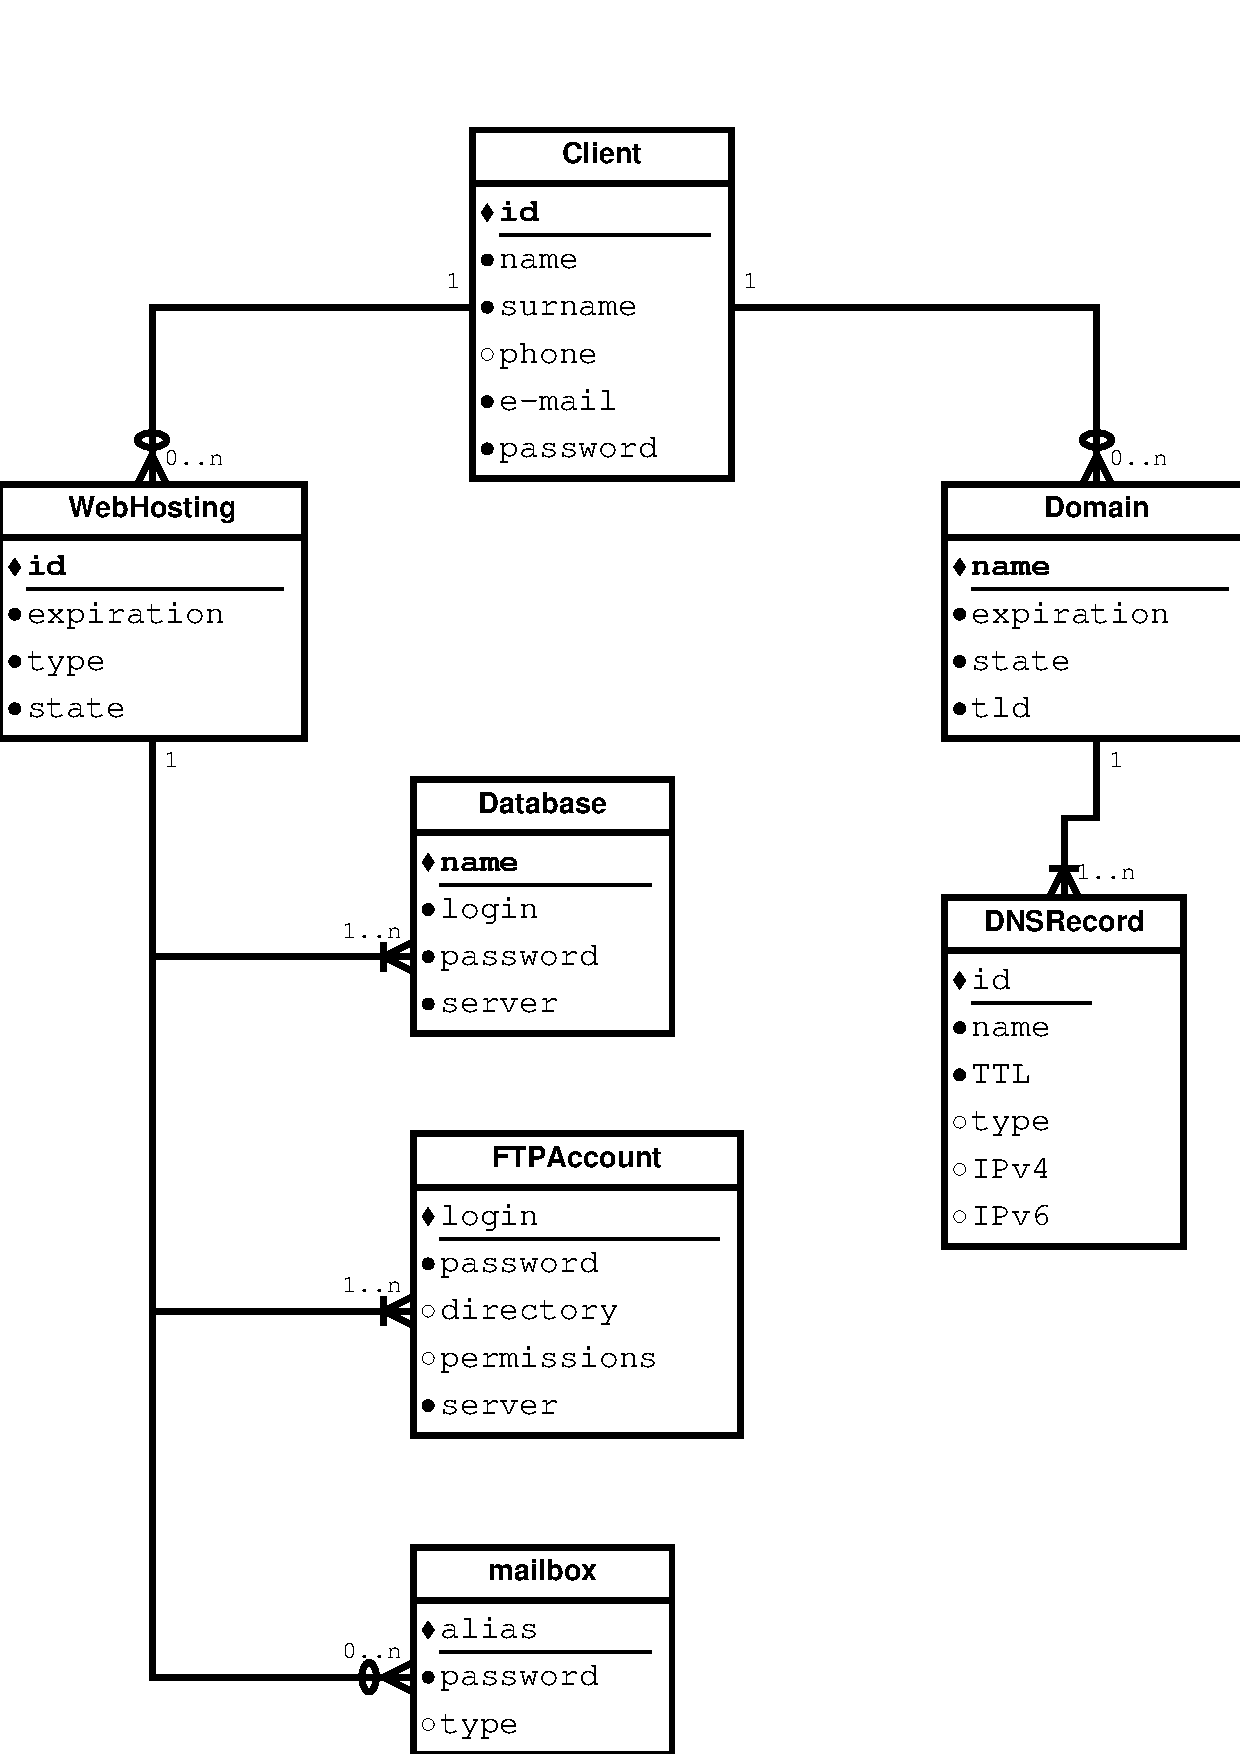
\includegraphics[width=10cm]{erd}
        \caption{ERD}
      \end{center}
    \end{figure}

\end{document}

